\chapter{Previsão de séries temporais com Regression WiSARD}
Como previsto no capítulo de redes neurais sem peso, o modelo Regression WiSARD é utilizado para resolver problemas de regressão, porém não é possível realizar previsão de séries temporais por depender de características que não são função do tempo. É possível, entretanto, tratar um problema de previsão de séries temporais como um problema de regressão aplicando técnicas como a janela deslizante e médias móveis conforme detalhado nas seções seguintes.

\section{Janelas deslizantes}
O método de janelas deslizantes é essencial para a Regression WiSARD ser capaz de realizar previsões de séries temporais. Isso ocorre porque é a técnica que permite transformar o problema temporal em um problema de regressão supervisionado.

O método consiste em tornar cada amostra dependente das $W$ amostras anteriores, e faz isso alocando uma janela de $W$ amostras no início da série temporal e deslocando até o final de amostra em amostra para formar a matriz de características, conforme ilustra a Figura~\ref{fig:sliding_window}, onde $W=3$ e $N$ é o número de registros da série temporal.

    \begin{figure}[!ht] \label{fig:sliding_window}
    \centering
    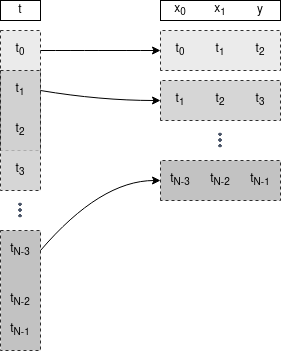
\includegraphics[width=3.0in]{img/sliding_window.png}
    \caption{Exemplo de aplicação do método de janelas deslizantes para transformar a série temporal $t$ em uma matriz de características $X$ e um vetor alvo $y$. }
    \end{figure}

Em alguns casos, também é possível utilizar outro parâmetro para a técnica, como o tamanho do passo da janela. No exemplo da Figura~\ref{fig:sliding_window}, esse tamanho foi considerado como $s=1$, já que o tamanho do passo para formar cada registro foi de 1.
% Exemplos práticos de utilização...

% Como ajuda na previsão de séries temporais com a Regression WiSARD...
\section{Média móvel}


% Exemplos práticos de utilização...

% Como ajuda na previsão de séries temporais com a Regression WiSARD...

\section{Regression WiSARD}
% Explicar treinamento do modelo...

% Explicar predições com o modelo...

% Vantagens - Aprendizado em tempo real, ...
